\documentclass[12pt,ngerman]{beamer}

\usepackage[utf8]{inputenc}
\usepackage[T1]{fontenc}
\usepackage{booktabs}
\usepackage{babel}
\usepackage{graphicx}
\usepackage{csquotes}
\usepackage{xcolor}

%\usetheme{AnnArbor}

\author{Uwe Ziegenhagen}
\title{EPUBs erzeugen mit LaTeX, lwarp und Calibre}
\subtitle{\url{github.com/UweZiegenhagen/TalksAndArticles}}

\usepackage{hyperref}
\usepackage{hyperxmp}
\hypersetup{%
   pdftitle={EPUBs erzeugen mit LaTeX, lwarp und Calibre},
   pdfauthor={Uwe Ziegenhagen},
   pdfcopyright={Copyright (C) 2017, Uwe Ziegenhagen. This work is licensed
under a Creative Commons Attribution-ShareAlike 4.0 International License},
   pdfsubject={Vortrag auf der Herbsttagung 2017 von DANTE e.V.},
   pdfkeywords={LaTeX,TeX,EPUB,DANTE e.V.},%ggf. anpassen
   pdflicenseurl={http://creativecommons.org/licenses/by-sa/4.0/},
   pdfcaptionwriter={},
   pdfcontactaddress={},
   pdfcontactcity={Cologne},
   pdfcontactpostcode={},
   pdfcontactcountry={Germany},
   pdfcontactphone={},
   pdfcontactemail={ziegenhagen@gmail.com},
   pdfcontacturl={www.uweziegenhagen.de},
   pdflang={de},
   pdfmetalang={de},
}

\begin{document}

\begin{frame}

\maketitle

\end{frame}

\begin{frame}
\frametitle{Inhalt}

\tableofcontents

\end{frame}

\section{Was ist eigentlich \enquote{EPUB}?}

\begin{frame}
\frametitle{Was ist eigentlich \enquote{EPUB}?}
\framesubtitle{Einführung}

Formate:

\begin{itemize}
	\item MOBI
	\item EPUB
\end{itemize}

EPUB:

\begin{itemize}
\item Akronym für \enquote{\textbf{e}lectronic \textbf{pub}lication}
\item offener Standard für E-Books 
\item International Digital Publishing Forum (IDPF)
\item ersetzt Open eBook (OEB/OEBPS) Standard
\item dynamische Anpassung des Textes an Ausgabegerät
\item kein Gerät implementiert Standard komplett
\end{itemize}

\end{frame}

\begin{frame}
\frametitle{Was ist eigentlich \enquote{EPUB}?}
\framesubtitle{Der EPUB Standard}

\textbf{Version 2}

\begin{itemize}
\item XML und XHTML,
\item DTBook, NCX, SVG, CSS,
\item Dublin Core und Zip,
\item sowie PNG, JPEG/JFIF, GIF
\end{itemize}

\textbf{Version 3}

\begin{itemize}
	\item ohne DTBook
	\item Medienüberlagerungen ($\Rightarrow$ Hörbuch)
	\item \enquote{Kanonische Fragmentidentifizierer} $\Rightarrow$ genaue Verweise
	\item Präsentation: seitenbasiert oder rollbar
\end{itemize}

\end{frame}

\section{Aufbau von EPUB-Dateien}

\begin{frame}
\frametitle{Aufbau von EPUB-Dateien}
\framesubtitle{Zerlegung einer EPUB-Datei}

\begin{itemize}
\item EPUB-Dateien sind Zip-Archive
%\item Siehe Beispiel von \url{http://www.inkshard.com/how-to-make-an-ebook-epub-file/}
%\item Validator unter \url{http://validator.idpf.org/}
\item \url{https://www.edrlab.org/epub/anatomy-of-an-epub-3-file/}
\item Aufbau:

\begin{description}
\item [mimetype] ''application/epub+zip''
\item [META-INF/] container.xml
\item [content.opf] DC-Informationen
\item [toc.ncx] Inhaltsverzeichnis
\item [\ldots] HTML, PNG/JPG, CSS 
\end{description}
\end{itemize}

\end{frame}

\section{Das \enquote{lwarp}-Paket}

\begin{frame}
\frametitle{Das \enquote{lwarp}-Paket}
\framesubtitle{~}

\begin{itemize}
\item Autor: Brian Dunn, \url{www.bdtech-concepts.com}
\item Sehr aktiv in der Entwicklung, seit 03/2016 über 40 Versionen
\item $\Rightarrow$ \TeX-Installation unbedingt vorher updaten
\item über 550 Seiten Dokumentation
\item  knapp 100 Seiten Nutzer-Doku
\end{itemize}

\end{frame}

\begin{frame}
\frametitle{Das \enquote{lwarp}-Beispiel}
\framesubtitle{~}

\begin{itemize}
\item Beispiel aus dem Handbuch (v39)
\item $\Rightarrow$ \texttt{lwarp-manual-example/example-01.tex}
\item Mit \texttt{pdflatex} übersetzen klappt 
\item Erzeugt verschiedenste Dateien: *.css, XDY, lwarpmk.conf, example-01\textunderscore html.tex, lwarp\textunderscore  mathjax.txt
\item Nutze das \texttt{lwarpmk} Tool:
\begin{itemize}
	\item \texttt{lwarpmk print}
	\item \texttt{lwarpmk html}
	\end{itemize}
\end{itemize}
\end{frame}

\begin{frame}
\frametitle{Ergebnisse von \texttt{lwarpmk html}}

\begin{center}
\fbox{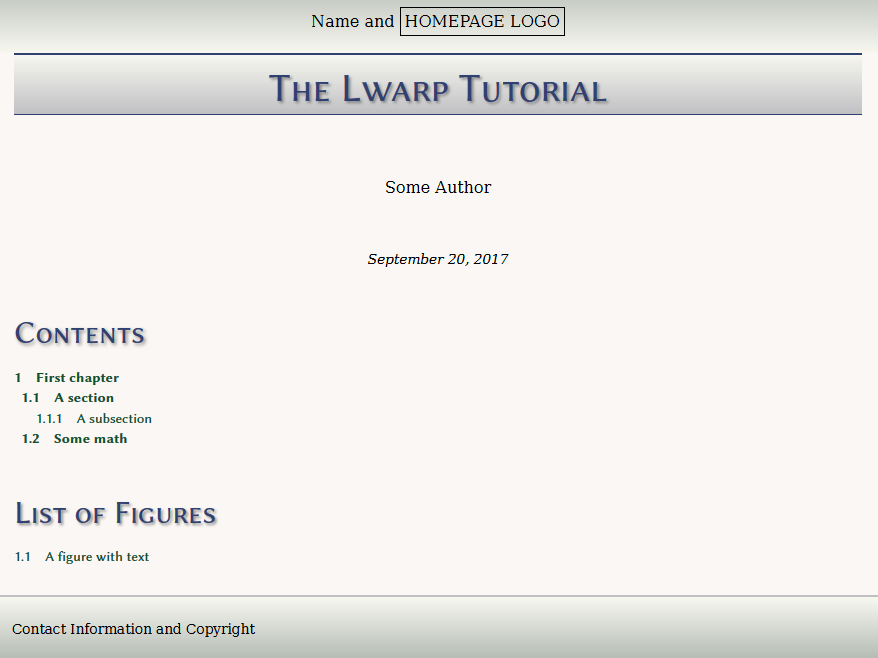
\includegraphics[width=0.8\textwidth]{lwarp-manual-example/bild-01.png}}
\end{center}

\end{frame}

\begin{frame}
\frametitle{Ergebnisse von \texttt{lwarpmk html}}

\begin{center}
\fbox{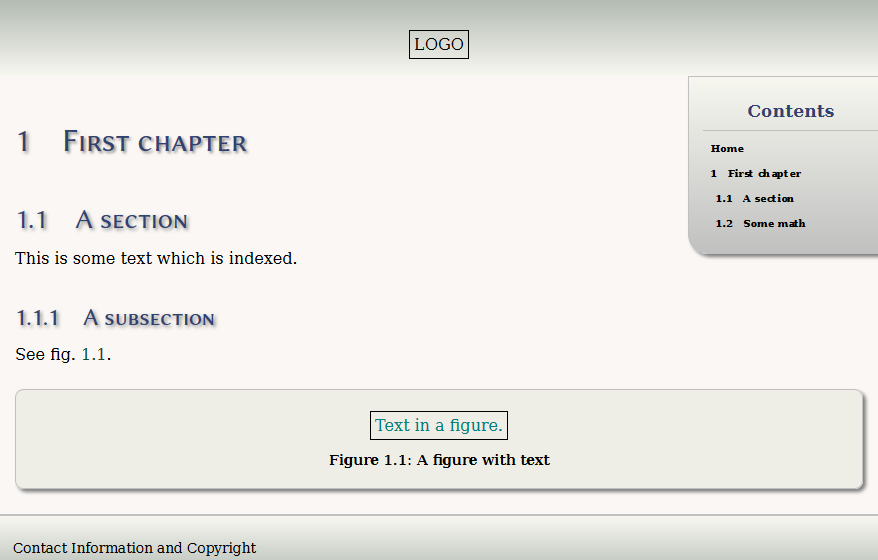
\includegraphics[width=0.8\textwidth]{lwarp-manual-example/bild-02.png}}
\end{center}

\end{frame}


\begin{frame}
\frametitle{Ergebnisse von \texttt{lwarpmk html}}

\begin{center}
\fbox{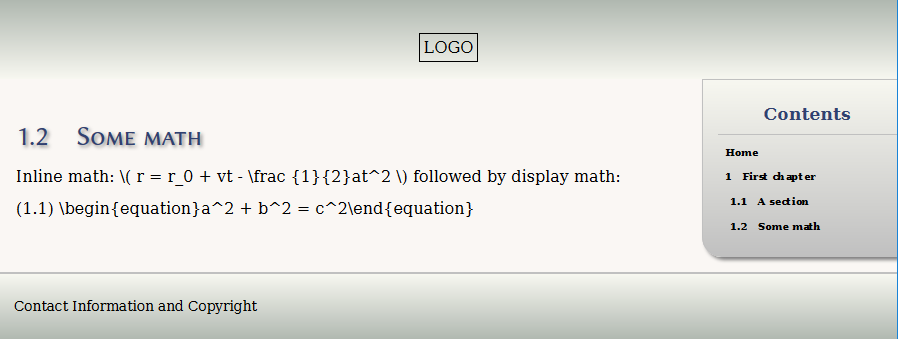
\includegraphics[width=\textwidth]{lwarp-manual-example/bild-03.png}}
\end{center}

\begin{itemize}
	\item Formeln fehlen
	\item Standard SVG $\Rightarrow$ \texttt{lwarpmk limages}
	\item Alternative Mathjax $\Rightarrow$ Paket-Option
\end{itemize}

\end{frame}

\section{Umwandlung nach EPUB}

\begin{frame}[fragile]
\frametitle{Umwandlung nach EPUB}
\framesubtitle{Anpassungen für EPUB}

\begin{itemize}
\item \verb|\booltrue{FormatEPUB}| in die Präambel
\item passt Kopf- und Fußzeilen sowie die Navigation an
\item sammelt die Fußnoten ein
\item danach \texttt{lwarpmk clean}
\item danach \texttt{lwarpmk html}
\end{itemize}
\end{frame}


\begin{frame}
\frametitle{Calibre}
\framesubtitle{Was ist Calibre?}

\begin{itemize}
\item Entwickler Kovid Goyal, seit 2006
\item \enquote{Eierlegende Wollmilchsau} der eBook-Verwalter
\item Verfügbar für alle gängigen Betriebssysteme
\item Katalogisierung und Verwaltung von elektronischen Büchern
\item Pflege von Metadaten
\end{itemize}
\end{frame}

\begin{frame}
\frametitle{Calibre}
\framesubtitle{GUI}

\begin{center}
\fbox{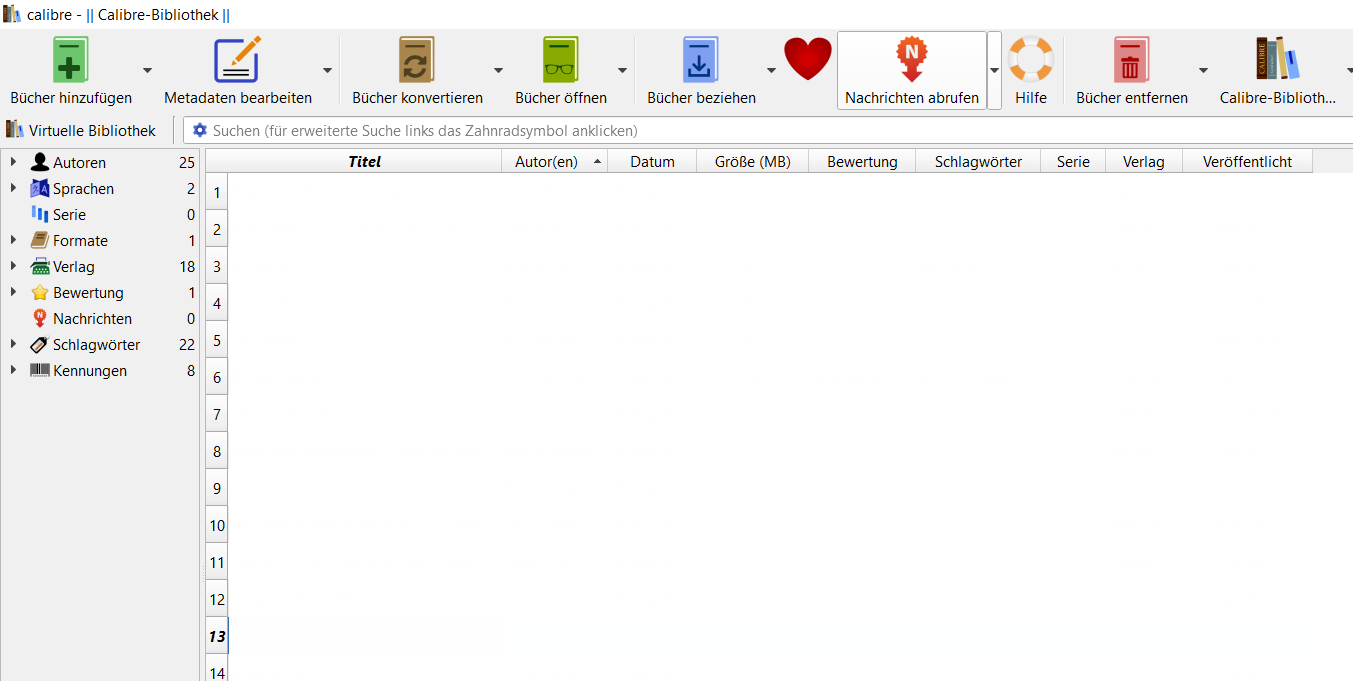
\includegraphics[width=\textwidth]{lwarp-manual-example/calibre-000.png}}
\end{center}

\end{frame}


\begin{frame}
\frametitle{Calibre}
\framesubtitle{Konfiguration}

\begin{center}
\fbox{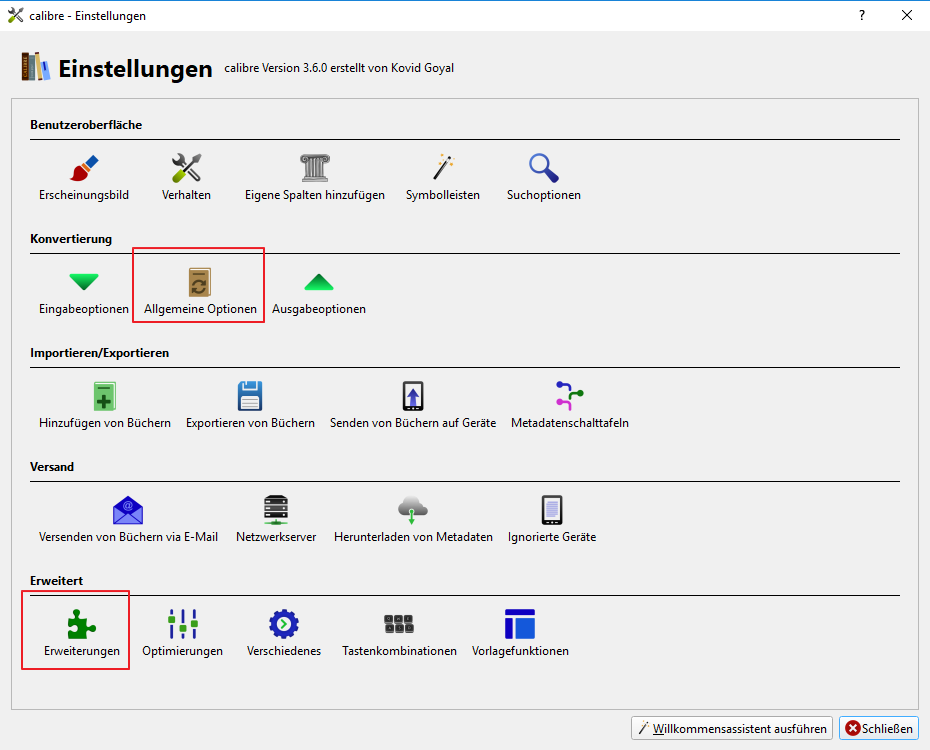
\includegraphics[width=0.8\textwidth]{lwarp-manual-example/calibre-00.png}}
\end{center}

\end{frame}

\begin{frame}
\frametitle{Calibre}
\framesubtitle{Konfiguration}

\begin{center}
\fbox{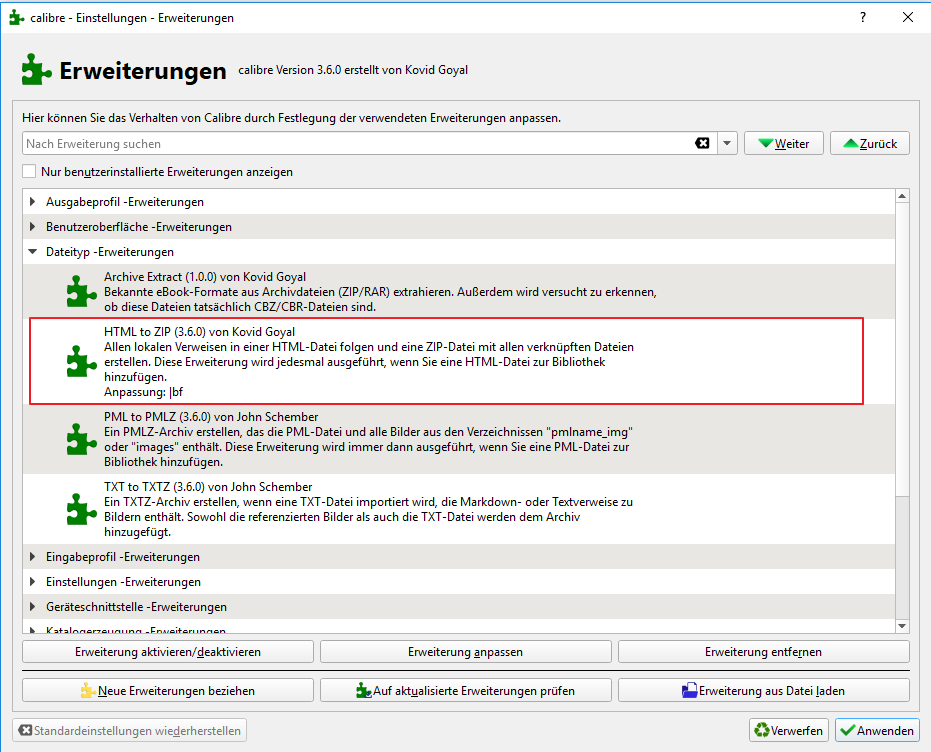
\includegraphics[width=0.8\textwidth]{lwarp-manual-example/calibre-01.png}}
\end{center}

\end{frame}


\begin{frame}
\frametitle{Calibre}
\framesubtitle{Konfiguration}

\begin{center}
\fbox{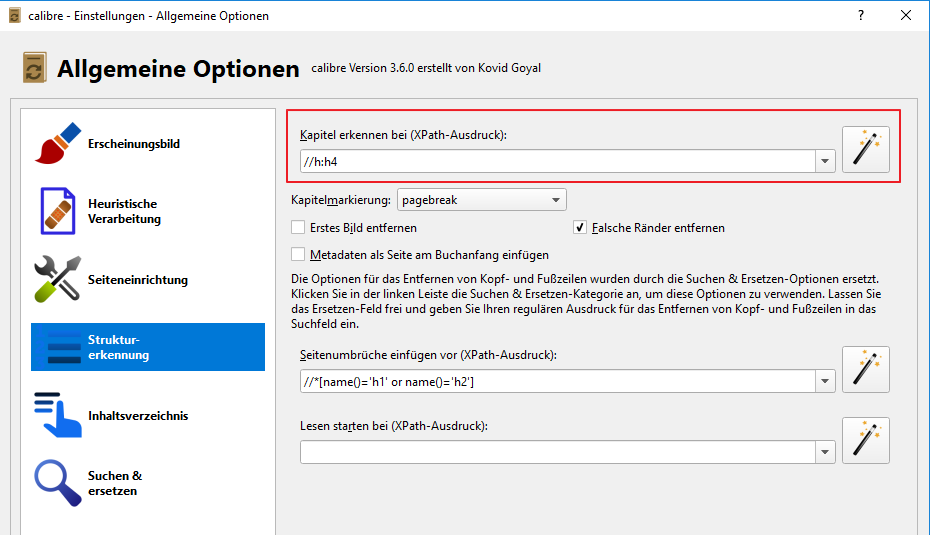
\includegraphics[width=0.9\textwidth]{lwarp-manual-example/calibre-02.png}}
\end{center}

\end{frame}



\begin{frame}
\frametitle{Eigenes Beispiel}
\framesubtitle{~}

\begin{itemize}
\item Bereinigung des Codes
\item KOMA-Klassen gehen nicht
\item \texttt{HomeHTMLFilename} and \texttt{HTMLFilename} gesetzt
\item Mit Blindtext gefüllt
\item Umwandlung mittels \texttt{lwarpmk html}
\end{itemize}
\end{frame}

\begin{frame}
\frametitle{Calibre}
\framesubtitle{Umwandlung}

\begin{itemize}
\item Hinzufügen eines Buches
\item Umwandlung und Export als EPUB
\item Ergebnisse:
\begin{itemize}
	\item Formeln nur unter iOS und Calibre Viewer
	\item Sumatra zeigt sie nicht
	\item werden aber nicht skaliert/gefärbt
\end{itemize}
\end{itemize}
\end{frame}

\begin{frame}
\frametitle{Fazit}
\framesubtitle{~}

\begin{itemize}
\item praktikabelste Möglichkeit, mit \LaTeX\ EPUBs zu erzeugen
\item Empfehlung: Testen am Anfang des Projekts
\end{itemize}
\end{frame}


\end{document}